\documentclass[12pt,a4paper]{amsart}

\usepackage[utf8]{inputenc}
\usepackage[english,russian]{babel}
\usepackage{a4wide}
\usepackage{tikz}
\usepackage{graphicx}
\usepackage{subcaption}

\usepackage[left=5cm,right=2cm, top=2cm,bottom=2cm,bindingoffset=0cm]{geometry}

\usepackage{anysize}
\usepackage{showkeys}

\newenvironment{comment}{}{}

\usepackage{hyperref}
\hypersetup{
  colorlinks   = true, %Colours links instead of ugly boxes
  urlcolor     = blue, %Colour for external hyperlinks
  linkcolor    = blue, %Colour of internal links
  citecolor   = red %Colour of citations
}

\newtheorem{proposition}{Предложение}[section]
\newtheorem{claim}{Утверждение}[section]
\newtheorem{conjecture}{Гипотеза}[section]
\newtheorem{corollary}{Следствие}[section]

\theoremstyle{definition}
\newtheorem{definition}{Определение}[section]
\theoremstyle{definition}
\newtheorem{designation}{Обозначение}[section]

% \newenvironment{theoremproof}
% {\par\noindent{\bf Доказательство Теоремы \arabic{section}.\arabic{theorem}}}
% {\hfill$\scriptstyle\blacksquare$}

\newenvironment{nouppercase}{%
  \let\uppercase\relax%
  \renewcommand{\uppercasenonmath}[1]{}}{}

\relpenalty=100
\binoppenalty=1000

\sloppy

% sections titling

\usepackage{etoolbox}
\patchcmd{\subsection}{\bfseries}{}{}{}
\usepackage{titlesec}
\titleformat{\section}[block]{\Large\bfseries}{}{-0.5em}{}
\titleformat{\subsection}[hang]{\large\bfseries}{}{0em}{}%\filcenter}{}{1em}{}
\titlespacing{\subsection}{0em}{2em}{1em}


% sections titling


% ToC

\setcounter{tocdepth}{3}
\makeatletter
\def\l@subsection{\@tocline{2}{0pt}{2.5em}{2em}{}}
%Make Chapter disapear in ToC
\renewcommand\tocchapter[3]{%
  \indentlabel{\@ifnotempty{#2}{\ignorespaces#2.\quad}}#3%
}
\newcommand\@dotsep{4.5}
\def\@tocline#1#2#3#4#5#6#7{\relax
  \ifnum #1>\c@tocdepth % then omit
  \else
    \par \addpenalty\@secpenalty\addvspace{#2}%
    \begingroup \hyphenpenalty\@M
    \@ifempty{#4}{%
      \@tempdima\csname r@tocindent\number#1\endcsname\relax
    }{%
      \@tempdima#4\relax
    }%
    \parindent\z@ \leftskip#3\relax \advance\leftskip\@tempdima\relax
    \rightskip\@pnumwidth plus1em \parfillskip-\@pnumwidth
    #5\leavevmode\hskip-\@tempdima{#6}\nobreak
    \leaders\hbox{$\m@th\mkern \@dotsep mu\hbox{.}\mkern \@dotsep mu$}\hfill
    \nobreak
    \hbox to\@pnumwidth{\@tocpagenum{#7}}\par
    \nobreak
    \endgroup
  \fi}
\makeatother
\AtBeginDocument{%
\makeatletter
\expandafter\renewcommand\csname r@tocindent0\endcsname{0pt}
\makeatother
}
\newcommand\atotoc[1]{\addtocontents{toc}{#1\par}}

\makeatletter
\def\l@section{\@dottedtocline{1}{1em}{1.5em}}
\makeatother


\apptocmd{\thebibliography}{\csname phantomsection\endcsname\addcontentsline{toc}{chapter}{Список литературы}}{}{}

% ToC

% headers and footers

\makeatletter
\def\ps@myPS{%
  \def\@oddfoot{\normalfont\scriptsize \hfil\rule{0pt}{20pt}\thepage\hfil
    \global\topskip\normaltopskip}%
    \let\@evenfoot\@oddfoot
  \def\@oddhead{\@serieslogo\hss}%
    \let\@evenhead\@oddhead % in case an article starts on a left-hand page
}
\makeatother

\pagestyle{myPS}

% headers and footers


% invisible section title

\newcommand{\invsection}[1]{
  \refstepcounter{section}%
  \addcontentsline{toc}{section}{\protect\numberline{\thesection}#1}%
  \sectionmark{#1}
}

% invisible section title

\newcommand{\E}{\mathrm{E}}
\newcommand{\hy}{\mu(X^l)}
\newcommand{\Exy}{\E_{x,y}}
\newcommand{\El}{\E_{X^l}}
\newcommand{\pd}[2]{\frac{\partial#1}{\partial#2}}
\newcommand{\Sum}{\sum\limits}
\renewcommand\i{\textit}
\renewcommand\t{\text}
\renewcommand\b{\textbf}
\newcommand\und\textunderscore


\setlength{\textwidth}{\paperwidth}
\addtolength{\textwidth}{-40mm}
\calclayout


\begin{document}

\begin{titlepage}

\begin{center}
Министерство образования и науки Российской Федерации
\vspace{0.4cm}

Федеральное государственное автономное образовательное учреждение высшего профессионального образования
\vspace{0.4cm}

<<Московский физико-технический институт (государственный университет)>>
\vspace{0.4cm}

Факультет инноваций и высоких технологий
\vspace{0.4cm}

Кафедра анализа данных
\vspace{0.7cm}

\end{center}
%\hrule

\begin{flushright}
  На правах рукописи

  УДК ????\phantom{}
\end{flushright}
%\hbox to \textwidth{
%\hss На правах рукописи}

\vspace{1.4cm}

\begin{center}
Левков Мирон Николаевич
\end{center}

\vspace{0.8cm}

\begin{center}
Гладкая метрика для задачи ранжирования
\end{center}

\vspace{1.3cm}

\begin{center}
\bf Выпускная квалификационная работа бакалавра
\end{center}

\vspace{1.8cm}

\begin{center}
Направление подготовки: 010400 Прикладные математика и информатика
\end{center}

\vspace{0.8cm}


\vspace{2.0cm}

Заведующий кафедрой \verb"              " \underline{\quad \quad \quad \quad \quad \quad \quad}
\verb"        "
/Бунина Е.И./

Научный руководитель \verb"              " \underline{\quad \quad \quad \quad \quad \quad \quad}
\verb"        "
/Воронцов А.С./

Студент \verb"                           " \underline{\quad \quad \quad \quad \quad \quad \quad}
\verb"        "
/Левков М.Н./

\vspace{1.0cm}

\hbox to \textwidth
{
\hss г. Москва \hss
}
\hbox to \textwidth
{
\hss 2017 \hss
}

\end{titlepage}

% ============================================================================================================

\title{Гладкая метрика для задачи ранжирования}

\author{М.Н.~Левков}


\begin{abstract}
Рассматривается задача ранжирования документов в поисковых запросах. В работе исследованы имеющиеся варианты сглаживания метрики ранжирования. Предложены различные способы сглаживания метрики DCG. Проведен анализ зависимости качества сглаженных метрик от гиперпараметров и размера выборки поисковых запросов.
\end{abstract}


\begin{nouppercase}
\maketitle
\end{nouppercase}

\tableofcontents

\pagebreak

% ============================================================================================================

\section{Введение}

\subsection{Описание задачи ранжирования}
Пусть имеется некий поисковый запрос. Задача ранжирования состоит в том, чтобы из списка всех доступных документов выбрать наиболее хорошие (релевантные) и показать их ползователю в поисковой выдаче. Для того, чтобы иметь возможность измерять качество алгоритма, выполняющего решение данной задачи, используются реальные оценки релевантности конкретных документов запросу, проставленные людьми.

\subsection{Обозначения}
\begin{designation}
Обозначим $\{d_i\}_{i=1}^n$ - набор \i{документов} релевантных данному поисковому запросу; 
$\{r_i\}_{i=1}^n$ - \i{рельные оценки} данных документов, проставленные ассесорами; \\
$\{s_i\}_{i=1}^n$ - оценки релевантности (\i{скоры}), выданные ранжирующим алгоритмом
\end{designation}

~\\

\begin{definition}
Метрика качества ранжирования \b{DCG} определяется по формуле:
$$DCG = \Sum_{i=1}^k \frac{r_{p_i}}{discount(i)}$$
где \\
$p_1,...,p_n$ - перестановка на множестве $\{1,...,n\}$, т.ч. ${s_{p_1} > s_{p_2} > ... > s_{p_n}}$ \\
k - количество документов, по которым считается метрика ($k \le n$) - важен в том случае, когда нас интересуют лишь несколько первых документов в выдаче \\
discount(i) - дисконтирующий фактор, как правило $\frac{1}{i}$ \\
\end{definition}

% ============================================================================================================
\newpage
\section{Постановка задачи}

Традиционные метрики ранжирования имеют конструкцию похожую на DCG: для подсчета метрики считается сумма по всем документам, \i{порядок} слагаемых в которой \i{зависит} от скоров, выданных ранжирующим алгоритмом, а \i{значения - нет}.\\


Несложно заметить, что для такой конструции при фиксированном наборе документов и их оценок данная метрика может принимать лишь конечное количество различных значений. При этом изменение значения метрики происходит лишь в случае перестановки местами двух документов в выдаче.\\

Как было замечено выше, основная проблема подобных метрик в том, что они не имеют гладкой зависимости от скоров. В то же самое время логично ожидать, что, если ранжирующий алгоритм выдал трем документам оценки $\{100, 1, 0.5\}$, а другим трем документам - $\{10, 1, 0.5\}$, то он считает первый документ из первой тройки сильно лучшим, чем первый документ из второй тройки. В добавок, гладкая относительно скоров метрика является более чувствительным инструментом для оценивания качества алгоритма и отслеживания случаев недообучения или переобучения.\\

В данной работе исследуются разные подходы к построению метрик ранжирования, с целью получения метрики, которая бы удовлетворяла ряду свойств, вводимых далее\\

% ============================================================================================================

\newpage
\section{Метрики качества результатов}

Хотелось бы, чтобы наша метрика обладала двумя свойствами. Во-первых, метрика должна быть "реалистичной". Т.е. ее локальные минимумы/максимумы должны соответствовать минимумам/максимумам DCG.
\begin{definition}
Пусть $\{y_i\}_{i=1}^k$ - значения метрики DCG на данном пуле запросов для k различных значений набора гиперпараметров. Пусть $\{\hat{y}_i\}_{i=1}^k$ - значения нашей метрики на том же пуле при тех же наборах гиперпараметров. Тогда \b{качеством аппроксимации} метрики DCG нашей метрикой назовем величину
$\underset{\alpha, \beta}{\min}\frac{1}{k}\Sum_{i=1}^k (y_i - \hat{y_i})^2$
\end{definition}

\begin{designation}
Далее будем обозначать \i{качество аппроксимации}, как $\t{approx(Metric Name)}$
\end{designation}

~\\

Также придуманная метрика должна быть гладкой. При этом необходим способ подсчета гладкости конкретной функции, если она задана не аналитически, а численно. Определим метрик гладкости.

\begin{definition}
Пусть $\{y_i\}_{i=1}^k$ - значения нашей метрики на данном пуле запросов для k различных значений набора гиперпараметров. Тогда \b{гладкостью} функции, посчитанной \b{через усреднение модуля разности} в соседних точках, будем называть величину 
$$\t{smooth}_\t{abs}(y_1,...,y_k) = \Sum_{i=2}^k |y_i - y_{i-1}| \cdot \frac{1}{|y_k - y_1|}$$
\end{definition}

\begin{definition}
Пусть $\{y_i\}_{i=1}^k$ - значения нашей метрики на данном пуле запросов для k различных значений набора гиперпараметров. Тогда \b{гладкостью} функции, посчитанной \b{через нормировку дисперсии} разности в соседних точках, будем называть величину 
$$\t{smooth}_\t{std}(y_1,...,y_k) = \frac{\t{diff}_{std}}{|\t{diff}_{mean}|}$$
Здесь ~~~ $\t{diff}_{mean} = \frac{1}{k - 1} \Sum_{i=2}^k (y_i - y_{i-1})$, ~~~
$\t{diff}_{std} = \frac{1}{k - 1} \Sum_{i=2}^k (y_i - y_{i-1} - \t{diff}_{mean})^2$
\end{definition}

\begin{definition}
Пусть $\{y_i\}_{i=1}^k$ - значения нашей метрики на данном пуле запросов для k различных значений набора гиперпараметров. Пусть $window \in \mathbb{Z}, deg \in \mathbb{N}$. Тогда \b{гладкостью} функции, посчитанной \b{с помощью аппроксимации полиномами}, будем называть величину
$$\t{smooth}_\t{poly}(y_1,...,y_k) = \Sum_{i=1}^{k - window + 1} \frac{\left(poly_{deg}(y_i,...,y_{i + window - 1})_{i + \lfloor{\frac{window}{2}}\rfloor} - y_{i + \lfloor{\frac{window}{2}}\rfloor}\right)^2}{k - window}$$
Здесь ~~ $poly_{deg}(y_i,...,y_{i + window - 1})$ - аппроксимирующий полином степени deg, построенный по window точкам. Т.е. такой полином стпепени deg, что среднеквадратичное отклонение в точках $\{i,...,i + window - 1\}$ минимально.
\end{definition}

В терминах данных нами определений, новая метрика тем лучше, чем меньше такие показатели, как гладкость и аппроксимация.

Возникает ряд проблем с тем, что выбор конкретного способа измерения гладкости для сравнения наших метрик между собой неочевиден. Первая метрика хорошо отображает гладкость в том случае, если функция монотонна (если не учитывать шумовые колебания) - однако же в иных случаях данная метрика может быть плоха из-за нормировки на разность значений в крайних точках. 

Вторая метрика ведет себя лучше, однако тоже не является достаточно гибкой и интерпритируемой.

С последней метрикой встает проблема выбора параметров deg и window. Тем не менее эта метрика понятна и действительно способона достаточно хорошо отображать гладкость функции. После перебора разных вариантов выбор был сделан в пользу параметров ${deg = 4}$, ${window = 11}$. При этом стоит учитывать, что гладкость метрики ранжирования измерялась на множествах размера порядка 100 точек.

% ============================================================================================================

\newpage
\section{Метрика SoftDCG}

Рассмотрим  метрику SoftDCG. Данная метрика является попыткой сглаживания метрики DCG. Кратко разберем способ подсчета SoftDCG

Пусть наш набор документов в поисковом запросе уже упорядочен по скорам. Рассмотрим кокретный документ $d_j$ со скором $s_j$. Логично предположить, что скор не является точным определением того, на каком месте должен быть документ. Более точно: пусть ${s_j - s_{j + 1} < \varepsilon, s_{j - 1} - s_j > \varepsilon}$, тогда, если добавить к оценками ранжирующего алгоритма случайный шум с дисперсией $\varepsilon$, документы $s_j, s_{j+1}$ поменяются местами в выбаче более вероятно, чем $s_{j-1}, s_j$. Данный факт говорит о близости документов, однако DCG способен учитывать близость документов с точностью до 1 места.

\hspace*{-0.7cm}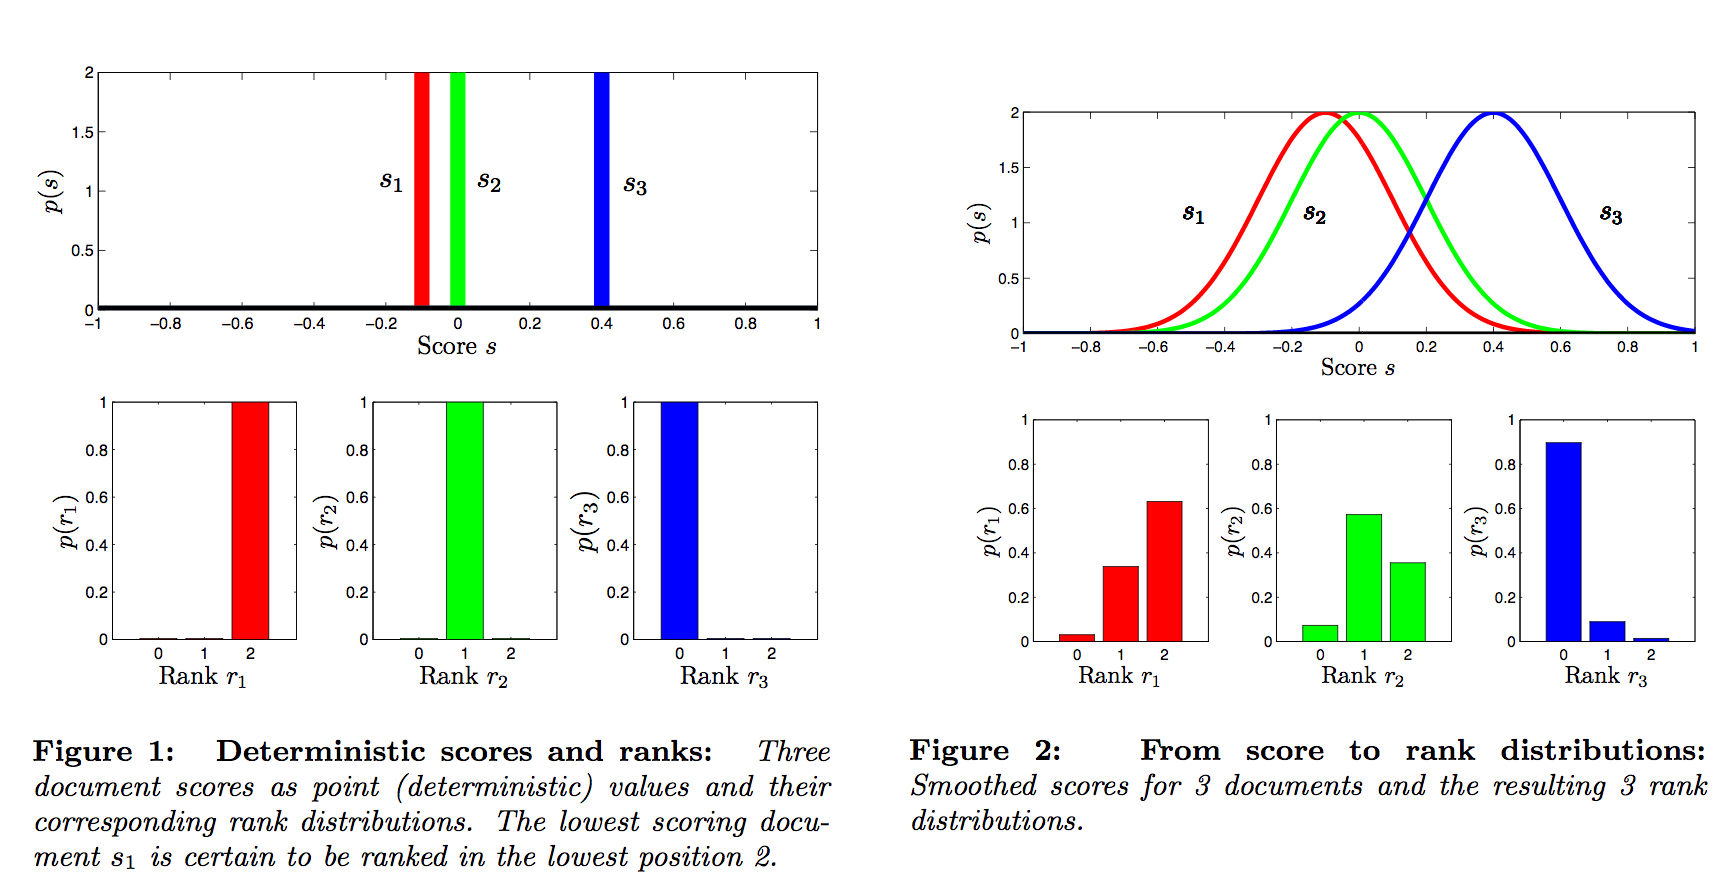
\includegraphics[width=0.85\paperwidth]{SoftDCG} \\

Метрика SoftDCG предполагает слудующее: вместо того, чтобы каждому документу сопоставлять конкретное место в поисковой выдаче, можно сопоставить ему нормальное распределение на местах. Параметры этого распределения подбираются по формулам исходя из скоров документов. Далее, зная распределение на местах, мы можем посчитать для каждого документа $$\hat{d}(j) = \E ~ \t{discount}(d_j) - \t{средний дискаунт j-го документа}$$.

Далее эти средние дискаунты используются для подсчета SoftDCG: $$\t{SoftDCG} = \Sum_{i=1}^n \hat{d}_j \cdot r_j$$

% ============================================================================================================

\newpage
\section{Метрика NoisedSoftDCG}

Рассмотрим другую метрику (назовем ее NoisedSoftDCG). Идея данной метрики берет свое начало в статье про SoftDCG, однако способ подсчета данной метрики несколько иной. \\

В SoftDCG каждому документу сопостовлялось некоторое вероятностное распределение на множестве возможных занимаемых позиций. При этом следует отметить, что данное распределение вполне четко задавалось аналитически. Благодаря этому имелась возможность задать такой параметр, как $\hat{d}(j)$ (средний дискаунт), формулой. \\

В данном же случае при подсчете метрики принимается во внимание лишь тот факт, что при небольшом изменении скоров на случайные величины значение метрики может меняться в силу того, что близкие документы будут переставляться местами. \\

Алгоритм подсчета NoisedSoftDCG следующий:

\begin{enumerate}
\item Получим скоры ранжирующего алгоритма $s_1,...,s_n$
\item Сгенерируем случайный шум $\xi_1,...,\xi_n$
\item $\hat{s}_1=s_1 + \xi_1,...,\hat{s}_n=s_n + \xi_n$
\item Посчитаем значение метрики $Value_{DCG}$
\item Повторим шаги (2)-(4) достаточно большое количество раз (T) и вычислим 
$NoisedDCG = \Sum_{i=1}^T Value_{DCG}^i$
\end{enumerate}

~\\

Можно дать некую интуицию по поводу того, почему метрика считается именно так. При достаточно большом Т близкие документы будут часто меняться местами, а усреднение DCG при этом даст некий аналог среднего дискаунта. Таким образом ожидается, что при больших Т данная метрика будет вести себя хорошо в плане гладкости  


% ============================================================================================================

\newpage
\section{Метрика FairSoftDCG}

Еще один вариант метрики, идея которой схожа с NoisedDCG. Заметим, что, основываясь на скорах, выданных ранжирующим алгоритмом, можно ввести вероятностное распределение на перестановках всех документов. \\

При этом распределение вводится так, что $P(d_i \t{ выше } d_j) \sim e^{\sigma(s_j - s_i)}$ (данное распределение можно ввести единственным образом). Благодаря этому для каждой перестановки на документах $p_1,...,p_n$ можно посчитать ее вероятность:
$$P(p_1,...,p_n) = \prod\limits_{i=1}^{n - 1} \frac{e^{\sigma s_{p_i}}}{\Sum_{k=j}^n e^{\sigma s_{p_j}}}$$

Теперь перебрав все перестановки документов можно посчитать "честное" мат. ожидание DCG. Собственно это у будет значением FairSoftDCG.
$$FairSoftDCG = \Sum_{p_1,...,p_n} P(p_1,...,p_n) \cdot DCG(p_1,...,p_n)$$

При этом возникает ряд проблем с данной метрикой, т.к. вычислительно данная задача достаточно сложная (всего имеется $n!$ возможных перестановок). В связи с этим был выбран способ подсчета близкого к данной метрике значения - подсчета по топ-k документам:
$$FairSoftDCG = \Sum_{p_1,...,p_k} P(p_1,...,p_k) \cdot DCG(p_1,...,p_k),$$ где сумма берется по всем возможным размещениям по k из n элементов


% ============================================================================================================

\newpage
\section{Применение результатов}

В данной части будут приведены предполагаемые способы использования искомой метрики. На данный момент идеальной - т.е. гладкой и хорошо аппроксимирующей DCG - метрики не найдено. Но следует учитывать, что любое небольшое улучшение метрики в смысле этих двух показателей является результатом. \\

Итак. Первый и способ применения более гладкой метрики - это использование ее в качестве инструмента показывающего качество обучения модели. Благодаря большей чувствительности появляется возможность следить за тем, как малые изменения гиперпараметров влияют на качество модели.

Простой пример: благодаря этой метрики можно достаточно хорошо измерять влияние новых элементов ансамбля в моделях градиентного бустинга. Точно так же можно использовать данную метрику для active learning like задач. Благодаря высокой чувствительности можно будет немного дообучать алгоритм на небольших частях датасета и смотреть на изменение качества ранжирования. \\

Второй и, пожалуй, самый важный с практической точки зрения способ применения нашей метрики - смешивание нескольких моделей ранжирования. В наши дни используются в ранжирующих системах крупных компаний используются абсолютно разные по характеру формулы. Эти формулы имеют разный масштаб выдаваемых значений. Каждая из этих формул придумывалась для оптимизации конкретной метрики - причем метрики могут быть кардинально различными по смыслу. При этом хотелось бы уметь смешивать формулы, выданные несколькими различными моделями, в один ансамбль формул, получая таким образом более мощную формулу ранжирования.

Данная проблема является достаточно трудоемкой и в терминах задачи ранжирования не решена. Т.к. наша метрика является гладкой и хорошо аппроксимирует DCG, оптимальная комбинация формул согласно этой метрике должна быть в той же окрестности, что и оптимум с точки зрения DCG. В то же самое время логично ожидать, что при взятии выпуклой комбинации двух формул должна получаться некая выпуклая гладкая кривая для значений метрики. \\

В качестве тривиального применения - добавления шума к скорам ранжирующего алгоритма. Здесь имеется ввиду следующее: если добавить к скорам модели шум с неким коэффициентом, это эквивалентно смешиванию двух моделей - нормальной и абсолютно бесполезной. Логично полагать, что оптимум качества в данном случае будет при коэффициенте, с которым берется шум, равном 0 (или близком к 0). Данный способ применения гладкой метрики - своеобразная sanity-check.

% ============================================================================================================

\newpage
\section{Эксперименты}

\subsection{Зависимость гладкости от размера пула запросов}
\pagebreak

% ============================================================================================================

\subsection{Зависимость качества аппроксимации от размера пула запросов}
\pagebreak

% ============================================================================================================

\subsection{Изменение метрики при добавлении шума}
\pagebreak

% ============================================================================================================

\newpage
\section{Проблема выбора гиперпараметра}

% ============================================================================================================

\newpage
\section{Выводы}

% ============================================================================================================

\newpage

\begin{thebibliography}{1}

\bibitem{SoftDCGPaper} \href{https://www.microsoft.com/en-us/research/publication/softrank-optimising-non-smooth-rank-metrics/}
{M. Taylor, J. Guiver, S. Robertson and T. Minka. SoftRank: Optimising Non-Smooth Rank Metrics. Microsoft Research Cambridge, 2016}
\bibitem{LambdaMARTPaper} \href{https://www.microsoft.com/en-us/research/publication/from-ranknet-to-lambdarank-to-lambdamart-an-overview/}
{Christopher J.C. Burges. From RankNet to LambdaRank to LambdaMART. Microsoft Research Technical Report, 2010}

\end{thebibliography}

% \begin{figure}[!h]
%     \centering
%     \begin{subfigure}{0.45\textwidth}
%     \centering
%         \includegraphics[height=2in]{MCF=1-n+2.png}
%         \caption{Пример $MCF(\mu,A)=\frac{2}{n+2}$}
%     \end{subfigure}
%     \centering
%     \begin{subfigure}{0.45\textwidth}
%     \centering
%         \includegraphics[height=2in]{triangle_homo.png}
%         \caption{Накрытие гомотетичным треугольником}
%      \end{subfigure}
% \end{figure}

\vspace{0.7cm}

\end{document}
